%THIS CODE IS MY OWN WORK, IT WAS WRITTEN WITHOUT CONSULTINGA TUTOR OR CODE WRITTEN BY OTHER STUDENTS - Jae Kyum Kim
\documentclass{article}
\usepackage{pythonhighlight}
\usepackage{graphicx}
\usepackage{subcaption}

\title{CS470 Homework 4}
\date{2020-04-09}
\author{Jaekyum Kim}

\begin{document}

  \pagenumbering{gobble}
  \maketitle
  \newpage
  \pagenumbering{arabic}
\paragraph{Collaboration Statement}
THIS CODE IS MY OWN WORK, IT WAS WRITTEN WITHOUT CONSULTING A TUTOR OR CODE WRITTEN BY OTHER STUDENTS - Jaekyum Kim

\section{Introduction}
The program is executable with 2 parameters: the name of the input graph file and the name of the output file. There are five different kinds of graph: 
graph1.dot: A graph with 5 vertices, with no dead ends nor spider traps.
graph2.dot: A graph with 10 vertices, with no dead ends nor spider traps.
graph3.dot: A graph with 10 vertices, with one dead end and no spider traps.
graph4.dot: A graph with 10 vertices, with one spider trap and no dead ends.
graph5.dot: A graph with 50 vertices, which may or may not contain dead ends and/or spider traps.
\section{How the Algorithm Works}

\begin{python}
for i in range(1,len(lineReadStrings)-1):
    tmp = lineReadStrings[i].split(" -> ")
    source = str(tmp[0]).strip()
    target = str(tmp[1]).strip()
    
    incoming.setdefault(target,[]).append(source)
    outgoing.setdefault(source,[]).append(target)
    
for each in incoming.keys():
    pr[each] = 1/len(incoming.keys())
#set up complete now run iteration
\end{python}
To start the algorithm, I first counted how many types of vertices are present in the graph and first initialized the pagerank value to 1/size. I used the split function to divide the source vertices and the target by using split(). Then, for convenience, I stored two variables called incoming edges and outgoing edges for later use, which was a great help to make succinct code.
\begin{python}

    
while True:
    
    for eachLetter in incoming.keys():
        tmp = 0

        for eachIncoming in incoming[eachLetter]:
            tmp = tmp + pr[eachIncoming] / len(outgoing[eachIncoming])
            
        #damping factor
        tmp = (1-damping)/len(incoming.keys()) + damping*tmp
        pr_tmp[eachLetter] = tmp
    
    sortedTuple = sorted(pr.items(), key=itemgetter(1))
    sortedTuple_tmp = sorted(pr_tmp.items(), key=itemgetter(1))
    
    pr = dict(pr_tmp)

    orderedLetter = [i[0] for i in sortedTuple]
    orderedLetter_tmp = [i[0] for i in sortedTuple_tmp]
    
    #print("Iterated.")
    if orderedLetter == orderedLetter_tmp:
        #print("Results converged, exit.")
        break;
\end{python}
To briefly explain the main part of the PageRank algorithm, it used the simplest approach by calculating the pagerank of the source vertices for each candidates, and divided it by the amount of outgoing edges the source vertex has. and I calculate it for each letter, and iterate through until the result converges(does not change). To avoid the error of possibility of spider traps and dead end, I set the damping factor as 0.85 and multiplied the pagerank by 0.85 and added (1-0.85)/size to each pagerank value. This technique takes account for when a surfer visit page 1, he could continue visit next link from 1, or he could type an address to go to another page. 

    \newpage

\section{Graph Visualization and PageRank Value}

\begin{figure}[h!]
  \centering
  \begin{subfigure}[b]{.6\linewidth}
    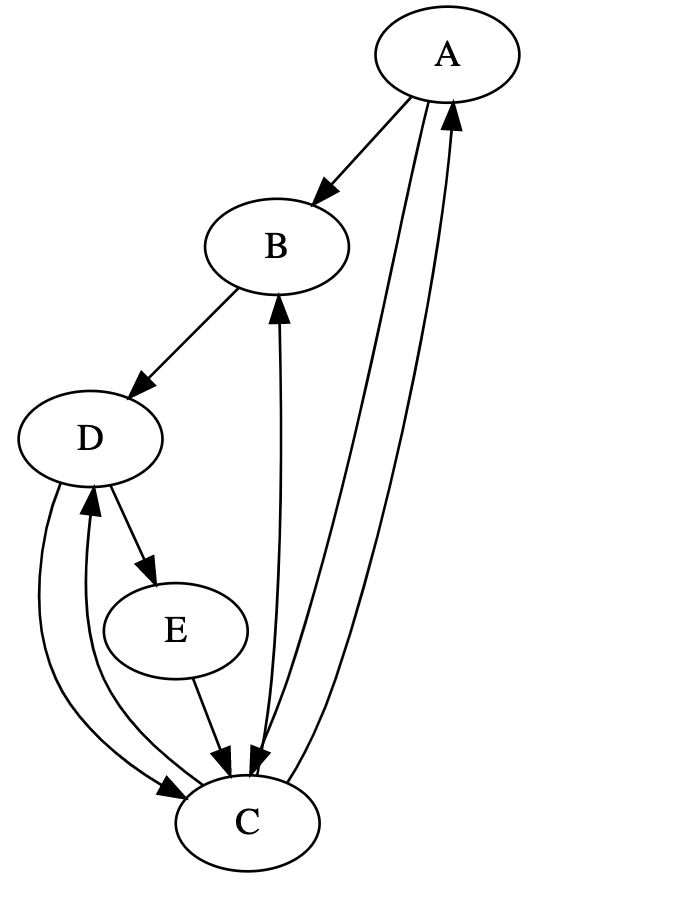
\includegraphics[width=\linewidth]{graph1.jpg}
  \end{subfigure}
  \caption{graph1}

  \end{figure}
  \paragraph{result}
 C,0.31
D,0.26
B,0.17
E,0.14
A,0.12

    \newpage

\begin{figure}[h!]
  \centering
  \begin{subfigure}[b]{.6\linewidth}
    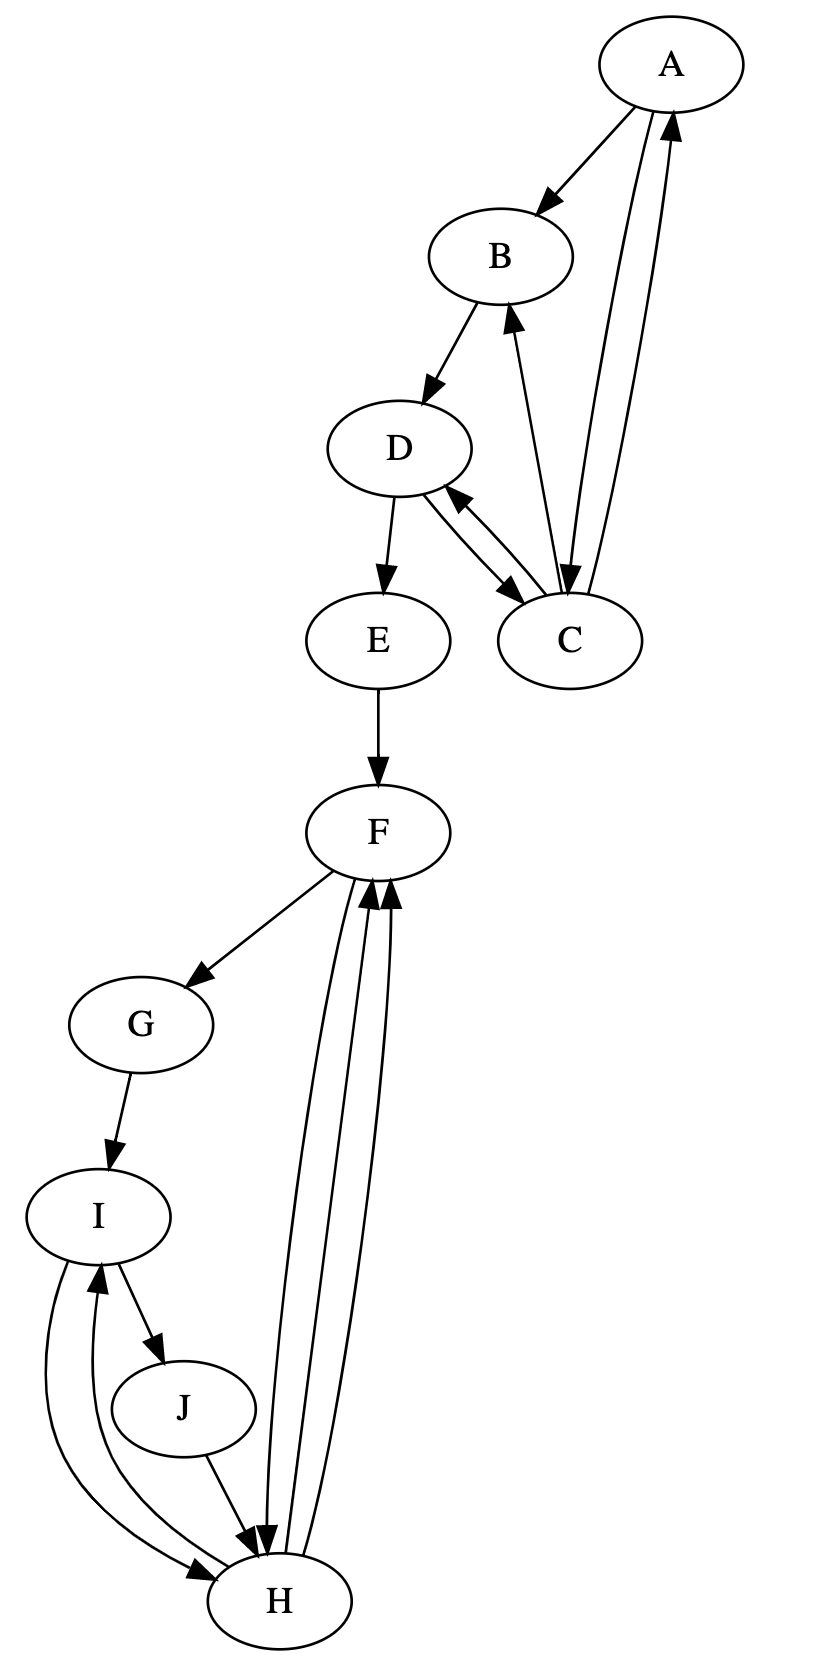
\includegraphics[width=\linewidth]{graph2.jpg}
  \end{subfigure}
  \caption{graph2 }

  \end{figure}
    \paragraph{result}

H,0.22
F,0.18
I,0.16
G,0.09
J,0.08
D,0.08
C,0.06
E,0.05
B,0.05
A,0.03
      \newpage

\begin{figure}[h!]
  \centering
  \begin{subfigure}[b]{.6\linewidth}
    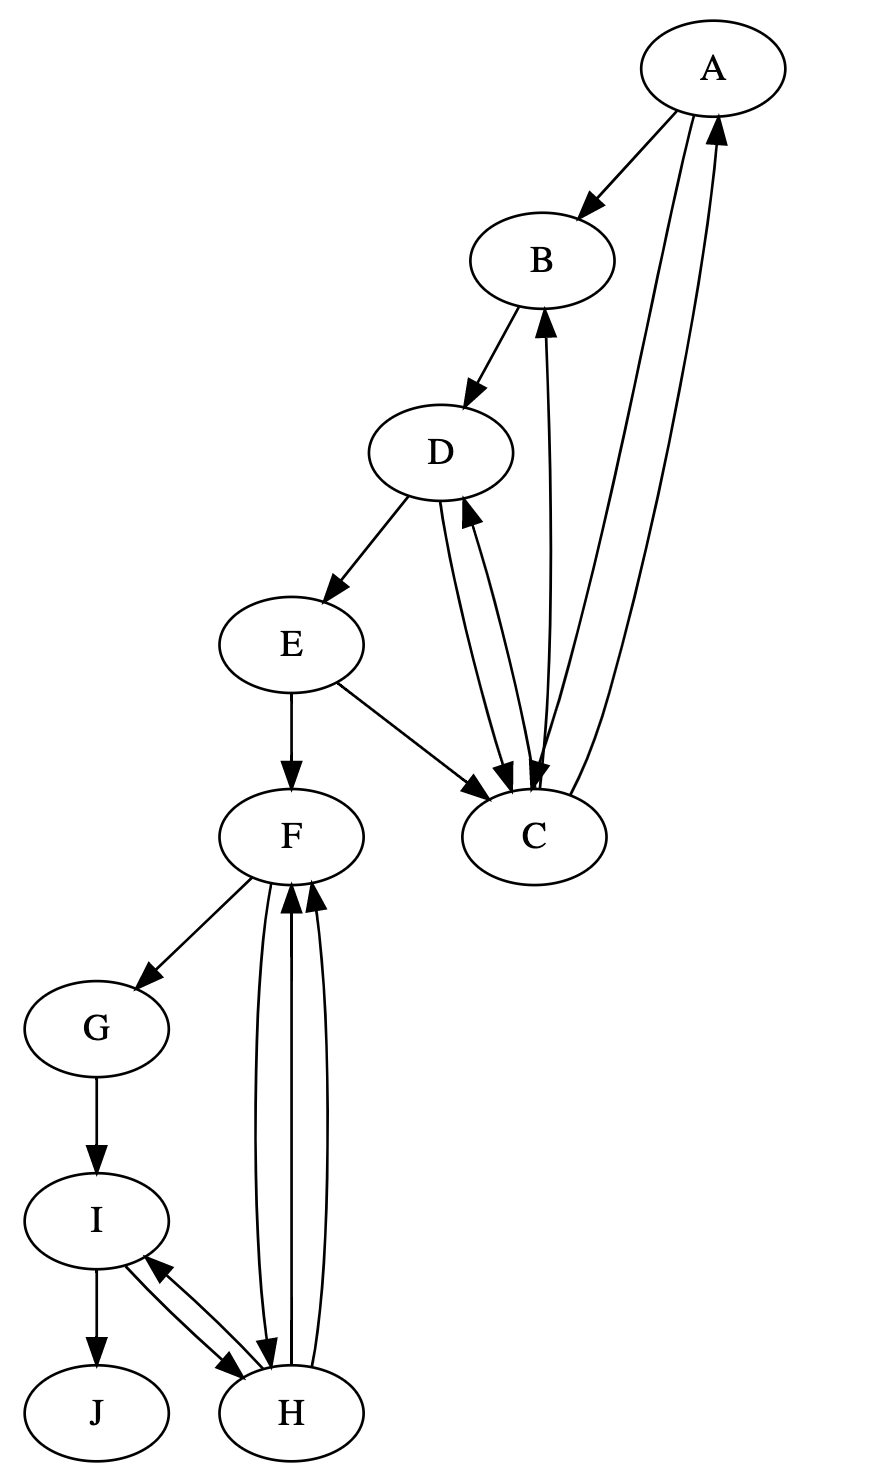
\includegraphics[width=\linewidth]{graph3.jpg}
  \end{subfigure}
  \caption{graph3 }

  \end{figure}
      \paragraph{result}

D,0.11
C,0.11
H,0.1
F,0.1
I,0.09
B,0.07
G,0.06
E,0.06
J,0.05
A,0.05
      \newpage

\begin{figure}[h!]
  \centering
  \begin{subfigure}[b]{.6\linewidth}
    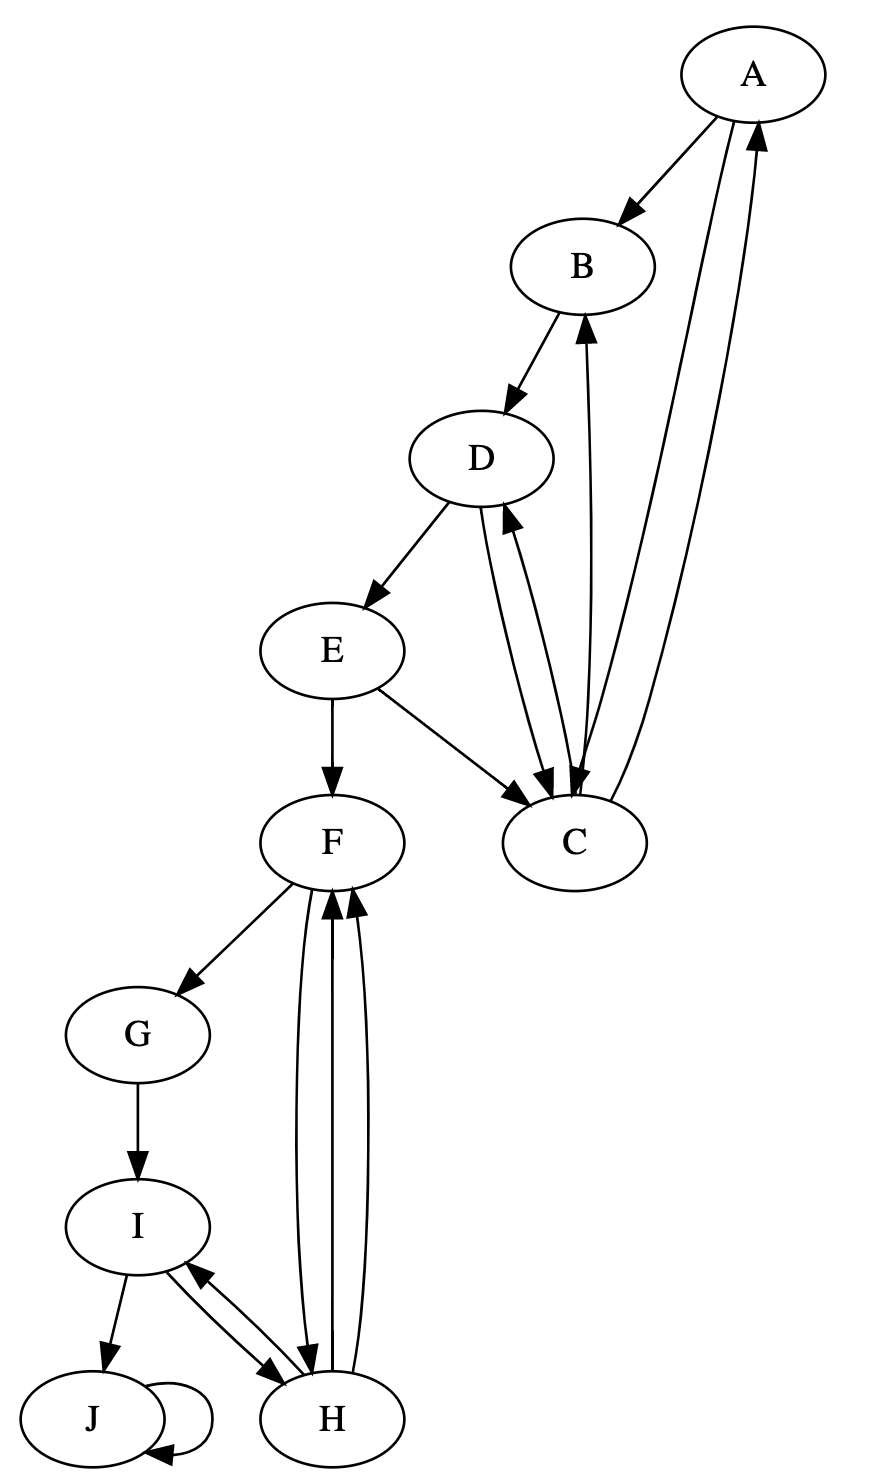
\includegraphics[width=\linewidth]{graph4.jpg}
  \end{subfigure}
  \caption{graph4}

  \end{figure}
        \paragraph{result}

J,0.26
D,0.11
C,0.11
H,0.1
F,0.1
I,0.09
B,0.07
G,0.06
E,0.06
A,0.05
      \newpage

\begin{figure}[h!]
  \centering
  \begin{subfigure}[b]{.05\linewidth}
    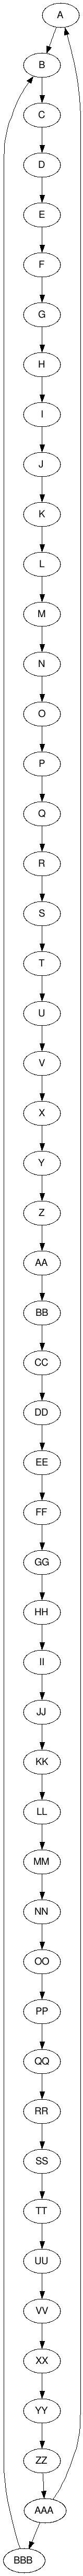
\includegraphics[width=\linewidth]{graph5.jpg}
  \end{subfigure}
  \caption{graph5}

  \end{figure}
  
        \newpage
        \newpage

          \paragraph{result for graph5}

B,0.021686801730183315\\
C,0.021314903846153848\\
D,0.021002283653846154\\
E,0.020736556490384615\\
F,0.020510688401442306\\
G,0.020318700525841345\\
H,0.020155510831580528\\
I,0.02001679959145883\\
J,0.019898895037355393\\
K,0.01979867616636747\\
L,0.019713490126027734\\
M,0.01964108199173896\\
N,0.0195795350775935\\
O,0.01952722020056986\\
P,0.019482752555099767\\
Q,0.019444955056450188\\
R,0.019412827182598045\\
S,0.019385518489823724\\
T,0.01936230610096555\\
U,0.019342575570436102\\
V,0.019325804619486072\\
X,0.019311549311178546\\
Y,0.01929943229911715\\
Z,0.01928913283886496\\
AA,0.0192803782976506\\
BB,0.019272936937618394\\
CC,0.01926661178159102\\
DD,0.019261235398967753\\
EE,0.019256665473737975\\
FF,0.019252781037292662\\
GG,0.019249479266314148\\
HH,0.01924667276098241\\
II,0.01924428723145043\\
JJ,0.01924225953134825\\
KK,0.0192405359862614\\
LL,0.019239070972937575\\
MM,0.01923782571161232\\
NN,0.019236767239485857\\
OO,0.019235867538178363\\
PP,0.019235102792066992\\
QQ,0.019234452757872327\\
RR,0.01923390022880686\\
SS,0.019233430579101214\\
TT,0.019233031376851416\\
UU,0.019232692054939087\\
VV,0.019232403631313608\\
XX,0.019232158471231952\\
YY,0.019231950085162545\\
ZZ,0.019231772957003547\\
AAA,0.019231622398068398\\
A,0.011058054903794454\\
BBB,0.011058054903794454\\
        \newpage


\end{document}



